%%%%%%%%%%%%%%%%%%%%%%%%%%%%%%%%%%%%%
\part{Preliminaries}
%%%%%%%%%%%%%%%%%%%%%%%%%%%%%%%%%%%%%

%%% --------------------------
\section{Motivation}
%%% --------------------------
\normalfont
\begin{frame}
	\begin{center}
  		\begin{alertblock}{Motivation} 
  			\begin{itemize}
  				\item Derive and convey key insights from data
  				\item Learn and use open source software
  				\item Explore first/another programming language
  				\item Gain ability to create insightful visualizations
  				\item Be more marketable 
  			\end{itemize}
		\end{alertblock}

	       \begin{center}
	         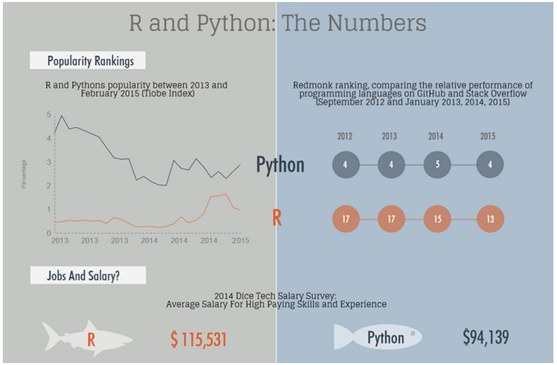
\includegraphics[scale=0.25]{images/r-vs-python-numbers}[6]
	        \end{center}

	\end{center} 
\end{frame}


%%% --------------------------
\section{Why R?}
%%% --------------------------
\begin{frame}
	\begin{center}
  		\begin{block}{Why R?} 
			\begin{itemize}
				\item Absolutely free!
				\item Used in industry and academia.
				\item Has a great community:
					\begin{itemize}
						\item StackOverflow
						\item Blogs
						\item Meetup groups
						\item MOOCs
						\item many, many others
					\end{itemize}
				\item Has over 7900 packages available for use (for free!).
				\item Transparent code (e.g. easier to check for bugs).
			\end{itemize}
		\end{block}
	\end{center} 
\end{frame}

%%% --------------------------
\section{Why visualize?}
%%% --------------------------
\begin{frame}
	\begin{center}
  		\begin{block}{Why visualize?} 
			\begin{itemize}
				\item \small Capture uncertainty in the data
				\item Explore potential relationships/trends/missing patterns (or absence thereof)
				\item Convey key information \normalfont
			\end{itemize}		
		\end{block}
	\end{center} 

   \begin{center}
     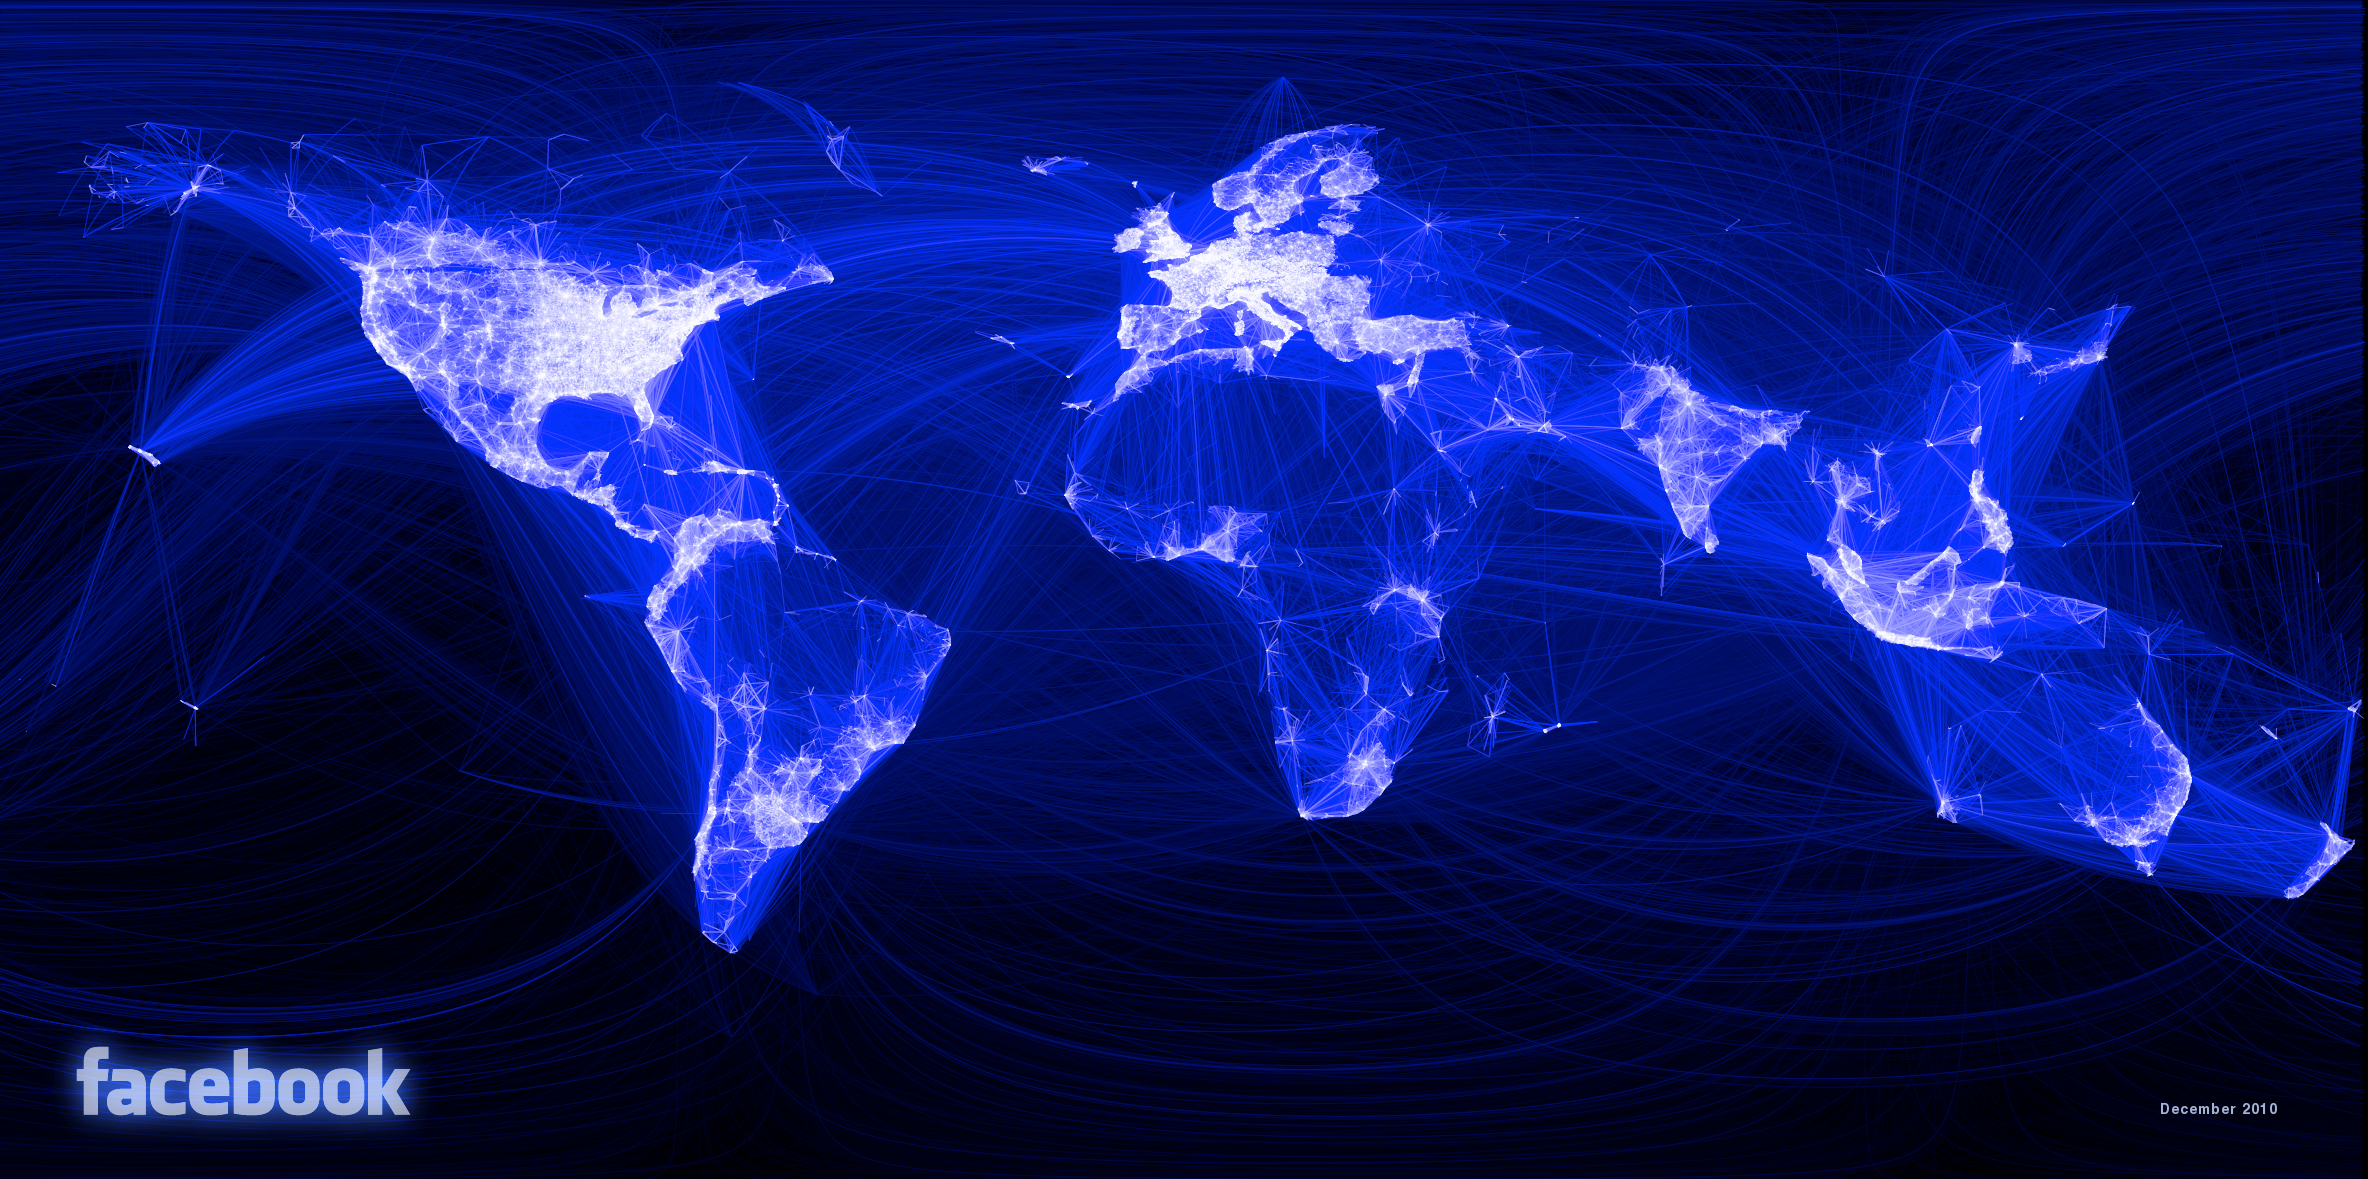
\includegraphics[scale=0.09]{images/facebook}[8]
    \end{center}

\end{frame}
%---

%%% --------------------------
\section{Tips for Visulizations}
%%% --------------------------
\begin{frame}
	\begin{center}
  		\begin{block}{Tips for visualizations} 
			\begin{itemize}
				\item Know your audience 
				\item \itshape{ 15 second rule:} \normalfont if your audience won't be able to understand the graphic in 15 seconds, simplify
				\item Color and font choices
				\item Add text/labels to figure
			\end{itemize}		
		\end{block}
	\end{center} 

  \begin{center}
  	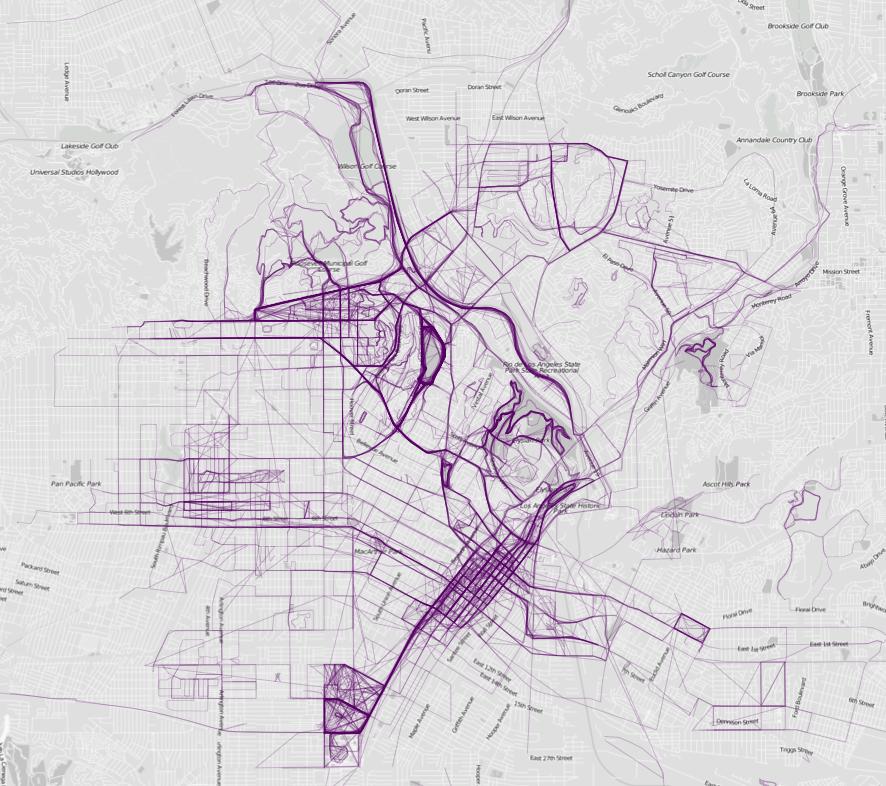
\includegraphics[width=0.4\textwidth]{images/geolocation_ex2}[7]
  \end{center}

\end{frame}
%---




%%%%%%%%%%%%%%%%%%%%%%%%%%%%%%%%%%%%%
\part{Introduction to R}
%%%%%%%%%%%%%%%%%%%%%%%%%%%%%%%%%%%%%

%%% --------------------------
\section{Overview of R}
%%% --------------------------
\begin{frame}
	\begin{center}
  		\begin{block}{Overview of R per John Chambers [1]:} 
			"To understand computations in R, two slogans are helpful:
			\begin{itemize}
			        \item Everything that exists is an object.
			        \item Everything that happens is a function call."
			\end{itemize}
		\end{block}
	\end{center} 

% R is flexible: 
% 	\begin{itemize}
% 		\item Objects can be variables, data sets, etc. and can be self-created, downloaded off the web (or elsewhere) and loaded from package(s).
% 		\item Functions (which do something to objects) can also be self-created, downloaded off the web (or elsewhere) and loaded from package(s).
% 		\item A package (1 of 7500+) is a collection of data sets and/or functions unified with a common theme.
% 	\end{itemize}
\end{frame}

%%% --------------------------
\subsection{Creating Objects}
%%% --------------------------
\begin{frame}
		\begin{block}{Creating objects in R}
Objects can be created in different ways, via:
			\begin{itemize}
				\item equal sign: \lstinline$ x = 3 $
				\item left arrow: \lstinline$ y <- 2 * x + 1 $
				\item right arrow: \lstinline$ 10 -> z $
			\end{itemize}
		\end{block}
\end{frame}

%%% --------------------------
\subsection{(Very) Brief Overview of Functions}
%%% --------------------------
\begin{frame}[fragile]
	\begin{center}
		\begin{block}{Function by example}
			\begin{lstlisting}[ basicstyle=\tiny]
f <- function(x, y=1){
	answer <- x * 2 + y + 1
	return(answer)
}

f(2)        # 6
f(3, 2)     # 9
f(y=3, 2)   # 8
f(y=3, x=3) # 10
			\end{lstlisting}	
		\end{block}

		\begin{block}{Components of a function:}
			\begin{itemize}
				\item Assign the function to a variable
				\item Add the 'function' keyword
				\item Specify any arguments (if any) that the function needs to compute the result
				\item Specify any argument defaults
			\end{itemize}
					%%% Assignment, arguments, named, order, unamed
		\end{block}
	\end{center} 
\end{frame}


\section{Working with Data}

\subsection{Reading Data from File}

%%%%%%%%%%%%%%%%%%%%%%%%%%%%%%%%%%%%%
% --------------------------------------------------- Slide --
\begin{frame}[fragile, allowframebreaks]
 \frametitle{Reading Data from File}

One approach is via \ttfamily read.table(). \normalfont  In the arguments of the function:
  \begin{itemize}
  \item \ttfamily file: \normalfont specifies the (relative) location, file name and file extension
  \item \ttfamily header: \normalfont if TRUE, tells R to include variables names when importing
  \item \ttfamily sep: \normalfont tells R how the entires in the data set are separated
    \begin{itemize}
      \item \ttfamily sep=",": \normalfont when entries are separated by COMMAS
      \item \ttfamily sep="$\backslash t$": \normalfont when entries are separated by TAB
      \item \ttfamily sep=" ": \normalfont when entries are separated by SPACE
    \end{itemize}
   \end{itemize}

\newpage   
   	\begin{lstlisting}[ basicstyle=\tiny]
filepath = "http://www.ats.ucla.edu/stat/data/test_missing_comma.txt"
### Other valid paths:
# filepath = "C:/Documents/test_missing_comma.txt"
# filepath = "./test_missing_comma.txt"
data <- read.table(
	file=filepath, 
	header=TRUE, 
	sep=","
	)
	\end{lstlisting}
\normalfont
\normalsize
\end{frame}

%%% --------------------------
\subsection{Working with Data Frames}
%%% --------------------------
\begin{frame}
	\frametitle{Working with Data Frames}
	To check that a data set has been read-in correctly: 
	\begin{itemize}
		\item View the first 5 lines of the dataset via \ttfamily head(): \normalfont \lstinline$ head(data, 5) $
		\item View the last 7 lines of the dataset via \ttfamily tail(): \normalfont \lstinline$ tail(data, 7) $
		\item Check the variable names via \ttfamily names(): \normalfont \lstinline$ names(data) $
		\item Check the size of the data set via \ttfamily dim(): \normalfont \lstinline$ dim(data) $
		\item Verify ranges and check for missing data via \ttfamily summary(): \normalfont \lstinline$ summary(data) $
	\end{itemize}
\end{frame}


%%% --------------------------
\section{Adding Functionality to Base R}
%%% --------------------------

\begin{frame}[fragile]
	\frametitle{Adding Functionality to Base R}

	\begin{itemize}
		\item Base R is what you download off CRAN \url{www.cran.r-project.org} 
		\item Available packages are listed here: \url{https://cran.r-project.org/web/packages/}
		\item Install an R package(s) via \ttfamily install.packages(): \normalfont 
   	\begin{lstlisting}
install.packages("ggplot2")
	\end{lstlisting}
	\end{itemize} 	
\end{frame}



%%%%%%%%%%%%%%%%%%%%%%%%%%%%%%%%%%%%%
